\documentclass[12pt]{article}

% -----------------------
% GEOMETRY --- ARTICLE 
\usepackage{geometry,setspace,hyperref}

\geometry{
	a4paper, % Paper size
	left	= 2.50 cm,
	right	= 2.50 cm,
	top		= 2.00 cm,
	bottom	= 2.00 cm,
	marginratio=1:1,
	%
	layoutvoffset	= 0.00 cm, 
	layouthoffset	= 0.00 cm, 
	%
	marginparwidth	= 2.00 cm, % So the 'todonotes' package doesn't flip out.
}

\pagestyle{empty} % Suppress page numbers 


\setstretch{1.30} % This is a good line spacing


% -----------------------


% -----------------------
% CONFIG PACKAGES
% -----------------------
% COLORS
\usepackage[dvipsnames]{xcolor}
\usepackage{amsmath}

% -----------------------
% TIKZ PACKAGES
\usepackage{tikz}
\usetikzlibrary{positioning}
\usetikzlibrary{calc,patterns,angles,quotes}%Tikz angles
\usetikzlibrary{decorations.text}
\usetikzlibrary{shapes.misc}
\usetikzlibrary{fadings}




% -----------------------
% CONFIG FONTS
%--------------------------
% Choose your font here
\usepackage{cmbright} 	% Sans-serif font similar to LaTeX default. Math mode looks good.
%\usepackage{kpfonts}	% Palatino-like font. Pretty

\usepackage{bm} % Make sure \boldsymbol works


%--------------------------
% Enabling \mathscr{} for pretty calligraphic fonts. :)

\makeatletter
\DeclareFontEncoding{LS1}{}{}
\DeclareFontEncoding{LS2}{}{\noaccents@}
\DeclareFontSubstitution{LS1}{stix}{m}{n}
\DeclareFontSubstitution{LS2}{stix}{m}{n}
\makeatother

\DeclareMathAlphabet\mathscr{LS1}{stixscr}{m}{n}
\SetMathAlphabet\mathscr{bold}{LS1}{stixscr}{b}{n}
\makeatother


% -----------------------
% EXTERNALISING FIGURES

\usetikzlibrary{external}
\tikzexternalize[prefix=./outputs/] % activate and define figures/ as cache folder
% Forced remake (only remakes things when code is changed). 
% If you change the config file, uncomment this once
%\tikzset{external/force remake}	

% -----------------------
% TIKZ-FEYNMAN

%Feynman Diagrams -- LuaLaTeX compiler needed
\usepackage[compat=1.1.0]{tikz-feynman}
\tikzfeynmanset{/tikzfeynman/warn luatex=false} % Except not really, you can turn off the warning

% Configuration file -- sets the default colours for TIKZ-FEYNMAN elements
%%%%%%%%%%%%%%%%%%%%%%%%%%%%%%%%%%%
% CONFIG FILE FOR TIKZ-FEYNMAN

% ----------------------
% Tikz-Feynman configurations:

% Shorter momentum arrows, farther from the diagram:
\tikzfeynmanset{/tikzfeynman/momentum/arrow distance=3.0mm}
\tikzfeynmanset{/tikzfeynman/momentum/arrow shorten= .30}

% ----------------------
% Momentum arrows in black by default
\tikzfeynmanset{momentum/arrow style = {Black}}


% ---------------------
% DEFINE GHOSTS TO HAVE ARROWS AND ROUND DOTS

\makeatletter
\tikzset{
	dot diameter/.store in=\dot@diameter,
	dot diameter=3pt,
	dot spacing/.store in=\dot@spacing,
	dot spacing=3pt,
	dots/.style={
		line width=\dot@diameter,
		line cap=round,
		dash pattern=on 0pt off \dot@spacing
	}
}
\makeatother

\tikzfeynmanset{
	ghost/.style={
    	/tikz/draw=none,
		/tikz/decoration={name=none},
		/tikz/postaction={
		/tikz/draw,
		/tikz/dots,		%Using /tikz/dots (defined above) instead of /tikz dotted
		/tikz/very thick,
		/tikzfeynman/with arrow=0.5, % Arrow at midpoint of edge
		},
	}
}



% ---------------------
% DEFINE BLOBS

\tikzfeynmanset{
	blob/.style={
		/tikz/shape	= circle,
		/tikz/draw	= black,			% Edge colour
		/tikz/fill	= gray!40,			% Interior colour
		% ---
		/tikz/inner sep 	= 0.25 cm,	% Separation between label and edge (I presume)
		/tikz/minimum size  = 2.00 cm,	% Minimum size, otherwise scales with label
	}
}


%---------------------
% ADD COLORS (OPIONAL)

\tikzfeynmanset{
	% A possible style:
	%gluon/.append style	= {RoyalBlue},
	%momentum/arrow style 	= {Red!80!Black},
	blob/.append style		= {/tikz/draw = RoyalBlue, /tikz/fill = RoyalBlue!20},
}







% -----------------------
% SOME COMMANDS

\newcommand{\mycomment}[1]{}

\newcommand{\sub}[1]{_{#1}^{}} %Subscripts with proper height
\newcommand{\upp}[1]{_{}^{#1}} %Superscripts with proper height
\newcommand{\ind}[2]{^{#1}_{#2}} %Both


%--------------------------
\begin{document}

\title{Tikz-Feynman Examples}
\author{André Cordeiro}
\date{April 2022}
\maketitle

%%%%%%%%%%%%%%%%%%%%%%%%%%%%%%%
\section{Outputs}

% ----------------------------------
\subsection{Document with Examples}

This document, compiled from \texttt{main-general.tex}, contains multiple examples of Feynman diagrams (particularly relevant for QCD). Each example is defined in a different \texttt{.tex} file in the \texttt{/inputs} directory, and included below.

For convenience, the \texttt{external} tikz library is used to export the outputs as individual \texttt{.pdf} files into the \texttt{/outputs} directory. An advantage of this library is that the \texttt{.tex} files are only compiled when changed, speeding up the compilation. To override this, uncomment the following line.
\begin{verbatim}
	\tikzset{external/force remake}	
\end{verbatim}

You should do this once after changing any of the configuration files, to ensure the changes take effect. Due to the externalisation, this file is useful to change the style of multiple figures at once.

Because the externalisation creates many files besides the \texttt{.pdf}, the \texttt{/outputs} directory contains a short script --- \texttt{clear.sh} --- to eliminate them.



% ----------------------------------
\subsection{Standalone}

The \texttt{main-standalone.tex} can be used to generate a single \texttt{.pdf} from one of the examples. This is useful to create images that change step by step.

The \texttt{.pdf} border can be adjusted by changing the first lines of \texttt{main-standalone.tex}.
\begin{verbatim}
	\documentclass[
	border={-10pt 0pt -6pt 0pt} % left bottom right top
	]{standalone} 
\end{verbatim}

Adjust in a case by case basis.

%%%%%%%%%%%%%%%%%%%%%%%%%%%%%%%
\section{Configuration Files}


% ----------------------------------
\subsection{Packages}

Simply includes the necessary \texttt{tikz} libraries necessary to draw the following examples.

% ----------------------------------
\subsection{Fonts}

In \texttt{config-fonts.tex} the font for the document can be changed. Here, two options are suggested, including \texttt{kpfonts} (a seriffed font which is slightly more distinctive than the \LaTeX\, default `Computer Modern') and \texttt{cmbright} (a sans-serif font fully compatible with math mode). Make sure to only uncomment one of these lines.

The \textbackslash\texttt{mathscr} commands were also defined, as an alternative to \textbackslash\texttt{mathcal}.

% ----------------------------------
\subsection{Tikz-Feynman}

In \texttt{config-feynman.tex}, the default styles were customised in different ways:

\begin{itemize}
	\item the momentum arrows are now shorter and coloured red,
	\item the \texttt{ghost} style uses both round dots and arrows (to distinguish `ghosts' from `antighosts'),
	\item the \texttt{blob} style is larger and coloured blue.
\end{itemize}

Other changes are possible, for example setting all photons to have a well defined colour, by adding the lines

\begin{verbatim}
\tikzfeynmanset{
	photon/.append style	= {yellow},
}
\end{verbatim}

to the end of the file. The different particle styles available in \texttt{tikz-feynman} are stated in its \href{https://ctan.org/pkg/tikz-feynman}{documentation}.

\newpage 

\section{Examples}

%%%%%%%%%%%%%%%%%%%%%%%%%%%%%%%%%%%
% THE QCD FEYNMAN RULES
%%%%%%%%%%%%%%%%%%%%%%%%%%%%%%%%%%%

\subsection{QCD Feynman Rules}

\begin{center}
	
% Set this figure's name when externalised 
\tikzsetnextfilename{qcdrules-vertex3gluon}
%
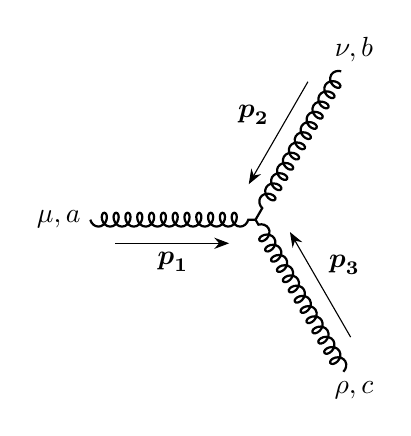
\begin{tikzpicture}

	% NOTE: MUST *NOT* INCLUDE A {} LABEL FOR THIS ONE
	%		IF A LABEL IS PROVIDED, THERE WILL BE A WHITE CIRCLE OVER THE VERTEX 
	%		USE \node FOR LABELS, \coordinate FOR NO LABEL
	\coordinate (C) at (0,0); 
	
	% Having specified the origin, 
	% the three endpoints are specified in polar coordinates:
	
	\node (V1) at (180:2.50cm) {\(\mu, a\)};
	\node (V2) at (+60:2.50cm) {\(\nu, b\)};
	\node (V3) at (-60:2.50cm) {\(\rho,c\)};
	
	%Pointless, except it extends the image into a square
	%\coordinate (Placeholder) at (0:2.50cm) {\phantom{\(\mu, a\)}};

	%%%%%%%%%%%%%%%%%%%%%%%%%%%%%%%%%%%%%%%%%%%%%%%%%%%%%%%%%%%%%%		
    \begin{feynman}

    %Diagram
    \diagram*{

    (V1) -- [thick, gluon, momentum' =\({ \boldsymbol{p_{1}^{}} }\)
    		,decoration={pre length=.00cm, post length=.05cm}
			] (C),

    (V2) -- [thick, gluon, momentum' =\({ \boldsymbol{p_{2}^{}} }\)
    		,decoration={pre length=.00cm, post length=.05cm}
            ] (C),

	%momentum' == arrow on the outside
    (V3) -- [thick, gluon, momentum' =\({ \boldsymbol{p_{3}^{}} }\)
    		,decoration={pre length=.00cm, post length=.05cm}
           	] (C),

    };
    
    \end{feynman}

\end{tikzpicture}

\tikzsetnextfilename{qcdrules-vertex4gluon} % Set this figure's name when externalised 
%
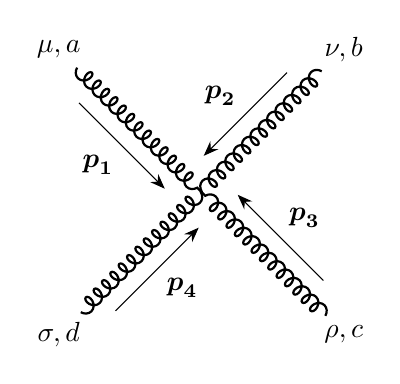
\begin{tikzpicture}

    
	% NOTE: MUST *NOT* INCLUDE A {} LABEL FOR THIS ONE
	%		IF A LABEL IS PROVIDED, THERE WILL BE A WHITE CIRCLE OVER THE VERTEX 
	%		USE \node FOR LABELS, \coordinate FOR NO LABEL
	\coordinate (C) at (0,0); 
	
	% Having specified the origin, 
	% the three endpoints are specified in polar coordinates:
	
	\node (V1) at (+135:2.56cm) {\(\mu, a\)};
	\node (V2) at ( +45:2.56cm) {\(\nu, b\)};
	\node (V3) at ( -45:2.56cm) {\(\rho,c\)};
	\node (V4) at (-135:2.56cm) {\(\sigma,d\)};
	
	%Pointless, except it extends the image into a square
	%\node (Placeholder) at (0:2.50cm) {\phantom{\(\mu, a\)}};
	
	%%%%%%%%%%%%%%%%%%%%%%%%%%%%%%%%%%%%%%%%%%%%%%%%%%%%%%%%%%%%%%		
    \begin{feynman}

    %Diagram
    \diagram*{

    %(C) -- [thick, gluon, rmomentum =\({ \boldsymbol{p_{1}^{}} }\)] (V1),
    %(C) -- [thick, gluon, rmomentum =\({ \boldsymbol{p_{2}^{}} }\)] (V2),
    %(C) -- [thick, gluon, rmomentum =\({ \boldsymbol{p_{3}^{}} }\)] (V3),
    %(C) -- [thick, gluon, rmomentum =\({ \boldsymbol{p_{4}^{}} }\)] (V4),

    (V1) -- [thick, gluon, momentum' =\({ \boldsymbol{p_{1}^{}} }\)] (C),
	(V2) -- [thick, gluon, momentum' =\({ \boldsymbol{p_{2}^{}} }\)] (C),
	(V3) -- [thick, gluon, momentum' =\({ \boldsymbol{p_{3}^{}} }\)] (C),
	(V4) -- [thick, gluon, momentum' =\({ \boldsymbol{p_{4}^{}} }\)] (C),


    };
    
    \end{feynman}
\end{tikzpicture}

% Set this figure's name when externalised 
\tikzsetnextfilename{qcdrules-vertexquarkgluon} 
%
\begin{tikzpicture}

	    
	% NOTE: MUST *NOT* INCLUDE A {} LABEL FOR THIS ONE
	%		IF A LABEL IS PROVIDED, THERE WILL BE A WHITE CIRCLE OVER THE VERTEX 
	%		USE \node FOR LABELS, \coordinate FOR NO LABEL
	\coordinate (C) at (0,0); 
	
	% Having specified the origin, 
	% the three endpoints are specified in polar coordinates: (angle:radius)
	
	\node (V1) at (180:2.50cm) {\(\mu, a\)};
	\node (V2) at (+60:2.50cm) {\(i\)};
	\node (V3) at (-60:2.50cm) {\(j\)};
	
	%%%%%%%%%%%%%%%%%%%%%%%%%%%%%%%%%%%%%%%%%%%%%%%%%%%%%%%%%%%%%%		
    \begin{feynman}

    %Diagram
    \diagram*{

	(V1) -- [thick, gluon] (C),
    
    (V3) -- [thick, fermion] (C)
         -- [thick, fermion] (V2),

    };
    
    \end{feynman}
\end{tikzpicture}

% Set this figure's name when externalised 
\tikzsetnextfilename{qcdrules-vertexghostgluon}
%
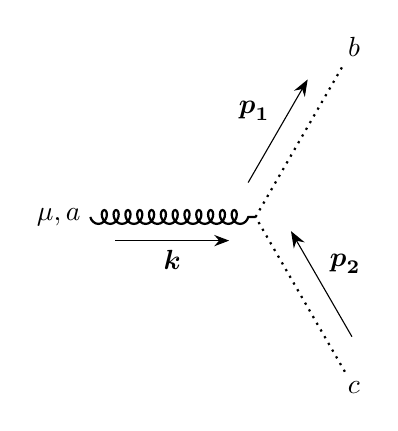
\begin{tikzpicture}

	
	% NOTE: MUST *NOT* INCLUDE A {} LABEL FOR THIS ONE
	%		IF A LABEL IS PROVIDED, THERE WILL BE A WHITE CIRCLE OVER THE VERTEX 
	\coordinate (C) at (0,0); 
	
	% Having specified the origin, 
	% the three endpoints are specified in polar coordinates:
	
	\node (V1) at (180:2.50cm) {\(\mu, a\)};
	\node (V2) at (+60:2.50cm) {\(b\)};
	\node (V3) at (-60:2.50cm) {\(c\)};	
	
	%%%%%%%%%%%%%%%%%%%%%%%%%%%%%%%%%%%%%%%%%%%%%%%%%%%%%%%%%	
    \begin{feynman}

    %Diagram
    \diagram*{

    (V1) -- [thick, gluon, momentum' =\({ \boldsymbol{k_{}^{}} }\)
			] (C),

    (C) -- [very thick, ghost, momentum =\({ \boldsymbol{p_{1}^{}} }\)
           ] (V2),

	%momentum' == arrow on the outside
    (V3) -- [very thick, ghost, momentum' =\({ \boldsymbol{p_{2}^{}} }\)
           	] (C),

    };
    
    \end{feynman}

\end{tikzpicture}

% Set this figure's name when externalised 
\tikzsetnextfilename{qcdrules-propagatorquark}
%
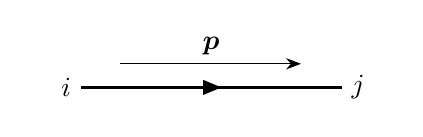
\begin{tikzpicture}

	%Vertices
	\node (Beg) {\(\hphantom{\mu,}i\)};
	
	\node (V1) at (4.00cm,0.00cm) {\(j\hphantom{\nu,}\)};
	
	%%%%%%%%%%%%%%%%%%%%%%%%%%%%%%%%%%%%%%%%%%%%%%%%%%%%%%%%%	
 	\begin{feynman}
    	
    %Diagram
    \diagram*{

    (Beg) -- [thick, fermion, momentum = \( \boldsymbol{p} \)] (V1), %momentum' == arrow on the outside

    };
    
    \end{feynman}
\end{tikzpicture}

% Set this figure's name when externalised 
\tikzsetnextfilename{qcdrules-propagatorgluon}
%
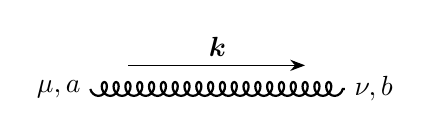
\begin{tikzpicture}

	%Vertices
	\node (Beg) {\(\mu, a\)};
	
	\node (V1) at (4.00cm,0.00cm) {\(\nu, b\)};

	%%%%%%%%%%%%%%%%%%%%%%%%%%%%%%%%%%%%%%%%%%%%%%%%%%%%
	\begin{feynman}
    
    %Diagram
    \diagram*{

    (Beg) -- [thick, gluon, momentum = \( \boldsymbol{k} \)] (V1), %momentum' == arrow on the outside

    };
    
    \end{feynman}
\end{tikzpicture}

% Set this figure's name when externalised 
\tikzsetnextfilename{qcdrules-propagatorghost} 
%
\begin{tikzpicture}

	%Vertices
	\node (Beg) {\(\phantom{\mu,}a\)};
	
	\node (V1) at (4.00cm,0.00cm) {\(b\phantom{\nu,}\)};

	%%%%%%%%%%%%%%%%%%%%%%%%%%%%%%%%%%%%%%%%%%%%%%%%%%%%
    \begin{feynman}

    %Diagram
    \diagram*{

    (Beg) -- [very thick, 
              ghost, % See config-feynman.tex for re-definition of 'ghost'
              momentum = \( \boldsymbol{p} \)] (V1), %momentum' == arrow on the outside

    };
    
    \end{feynman}
\end{tikzpicture}

\end{center}


\newpage

%%%%%%%%%%%%%%%%%%%%%%%%%%%%%%%%%%%%%%
% LOOPS IN QCD
%%%%%%%%%%%%%%%%%%%%%%%%%%%%%%%%%%%%%%

\subsection{QCD Loops}

% NOT EXHAUSTIVE, JUST THE ONES NEEDED TO RENORMALISE THE THEORY

\begin{center}
	
% Set this figure's name when externalised 
\tikzsetnextfilename{qcdloops-quarkselfenergy} 
%
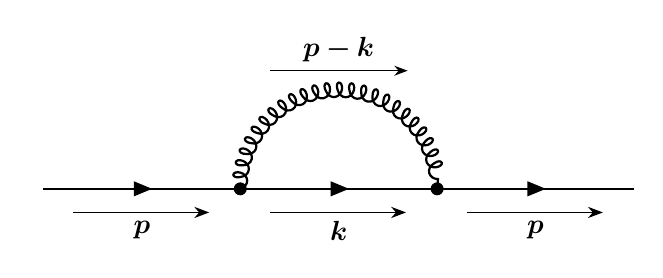
\begin{tikzpicture}
	
	\begin{feynman}

	% ------------------------------------------------
	% Ensure the dimensions of graphic are appropriate
	%\useasboundingbox (0, 0.7*\loopsh) rectangle (\loopsw, -0.3*\loopsh);
		
	% ------------------------------------------------
	% Relevant coordinates
	\coordinate (Beg) at (0.20cm,0);

	\path (Beg) +(2.50cm,0) coordinate (V1);
	\path (V1)  +(2.50cm,0) coordinate (V2);
	\path (V2)  +(2.50cm,0) coordinate (End);

	\path (V1)			+(0.00cm,1.20cm) coordinate (LabelStart);
	\path (LabelStart)	+(2.50cm,0.00cm) coordinate (LabelEnd);

	% ----------------
	% Dotted vertices
	\node[dot] (V1Dot) at (V1) +(0.00cm, 0.00cm);
	\node[dot] (V2Dot) at (V2) +(0.00cm, 0.00cm);
	
	%%%%%%%%%%%%%%%%%%%%%%%%%%%%%%%%%%%%%%%%%
    %Diagram
	\diagram*{
	
	(Beg)	-- [thick, fermion, momentum' = \(\boldsymbol{p}\)] (V1) 
			-- [thick, fermion, momentum' = \(\boldsymbol{k}\)] (V2)
			-- [thick, fermion, momentum' = \(\boldsymbol{p}\)] (End),
	
	(LabelStart) -- [opacity=0, momentum = \(\boldsymbol{p-k}\)] (LabelEnd)
	
	};

	\draw[thick, gluon] (V1) arc [start angle=180, end angle=0, radius=1.25cm];
		
	%\draw[blue, thick, gluon] (V1) arc [start angle=180, end angle=-180, radius=1.25cm];	
	
	\end{feynman}
	
\end{tikzpicture}

% Set this figure's name when externalised 
\tikzsetnextfilename{qcdloops-ghostselfenergy} 
%
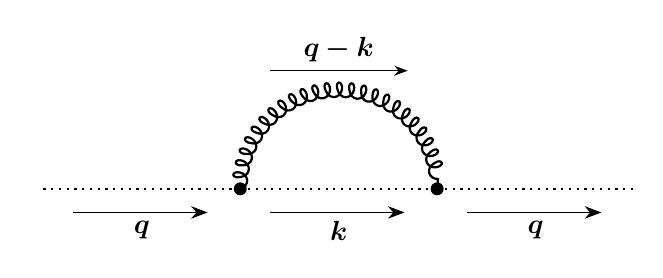
\begin{tikzpicture}
	
	\begin{feynman}	

	% ------------------------------------------------
	% Ensure the dimensions of graphic are appropriate
	%\useasboundingbox (0, 0.7*\loopsh) rectangle (\loopsw, -0.3*\loopsh);
	
	% ------------------------------------------------
	% Relevant coordinates
	\coordinate (Beg) at (0.20cm,0);
	
	\path (Beg) +(2.50cm,0) coordinate (V1);
	\path (V1)  +(2.50cm,0) coordinate (V2);
	\path (V2)  +(2.50cm,0) coordinate (End);
	
	\path (V1)			+(0.00cm,1.20cm) coordinate (LabelStart);
	\path (LabelStart)	+(2.50cm,0.00cm) coordinate (LabelEnd);
	
	% ----------------
	% Dotted vertices
	\node[dot] (V1Dot) at (V1) +(0.00cm, 0.00cm);
	\node[dot] (V2Dot) at (V2) +(0.00cm, 0.00cm);
	
	%%%%%%%%%%%%%%%%%%%%%%%%%%%%%%%%%%%%%%%%%
	%Diagram
	\diagram*{
		
		(Beg)	-- [very thick, ghost, momentum' = \(\boldsymbol{q}\)] (V1) 
				-- [very thick, ghost, momentum' = \(\boldsymbol{k}\)] (V2)
				-- [very thick, ghost, momentum' = \(\boldsymbol{q}\)] (End),
		
		(LabelStart) -- [opacity=0, momentum = \(\boldsymbol{q-k}\)] (LabelEnd),
		
	};
	
	\draw[thick, gluon] (V1) arc [start angle=180, end angle=0, radius=1.25cm];
	
	%\draw[blue, thick, gluon] (V1) arc [start angle=180, end angle=-180, radius=1.25cm];	
	
	\end{feynman}
	
\end{tikzpicture}

% Set this figure's name when externalised 
\tikzsetnextfilename{qcdloops-gluonloop} 
%
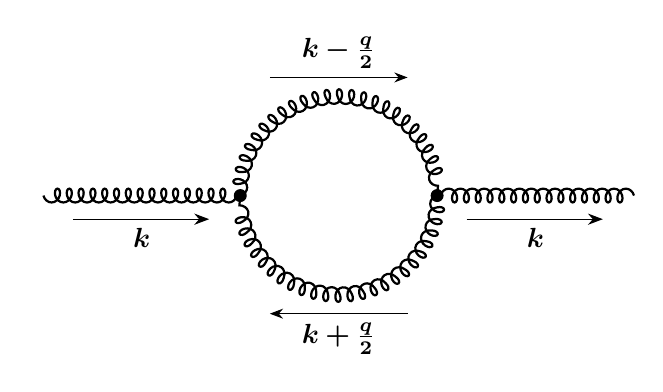
\begin{tikzpicture}

	\begin{feynman}
	
	% ------------------------------------------------
	% Ensure the dimensions of graphic are appropriate
	%\useasboundingbox (0, 0.7*\loopsh) rectangle (\loopsw, -0.7*\loopsh);
	
	% ------------------------------------------------
	% Relevant coordinates
	\coordinate (Beg) at (0.20cm,0);
	
	\path (Beg) +(2.50cm,0) coordinate (V1);
	\path (V1)  +(2.50cm,0) coordinate (V2);
	\path (V2)  +(2.50cm,0) coordinate (End);
	
	\path (V1)				+(0.00cm,1.20cm) coordinate (LabelStartUpper);
	\path (LabelStartUpper)	+(2.50cm,0.00cm) coordinate (LabelEndUpper);

	\path (V1)				+(0.00cm,-1.20cm) coordinate (LabelStartLower);
	\path (LabelStartLower)	+(2.50cm,0.00cm) coordinate (LabelEndLower);

	% ----------------
	% Dotted vertices
	\node[dot] (V1Dot) at (V1) +(0.00cm, 0.00cm);
	\node[dot] (V2Dot) at (V2) +(0.00cm, 0.00cm);

	%%%%%%%%%%%%%%%%%%%%%%%%%%%%%%%%%%%%%%%%%
	%Diagram
	\diagram*{
		
		(Beg)	-- [thick, gluon, momentum' = \(\boldsymbol{k}\)] (V1), 
		(End)	-- [thick, gluon, rmomentum = \(\boldsymbol{k}\)] (V2),
		
		(LabelStartUpper) -- [opacity=0, momentum = \(\boldsymbol{k-\frac{q}{2}}\)] (LabelEndUpper),
		
		(LabelStartLower) -- [opacity=0, rmomentum' = \(\boldsymbol{k+\frac{q}{2}}\)] (LabelEndLower),
		
	};
	
	\draw[thick, gluon] (V1) arc [start angle=180, end angle=0, radius=1.25cm];
	\draw[thick, gluon] (V2) arc [start angle=0, end angle=-180, radius=1.25cm];
	
			
	\end{feynman}
	
\end{tikzpicture}

% Set this figure's name when externalised 
\tikzsetnextfilename{qcdloops-quarkloop} 
%
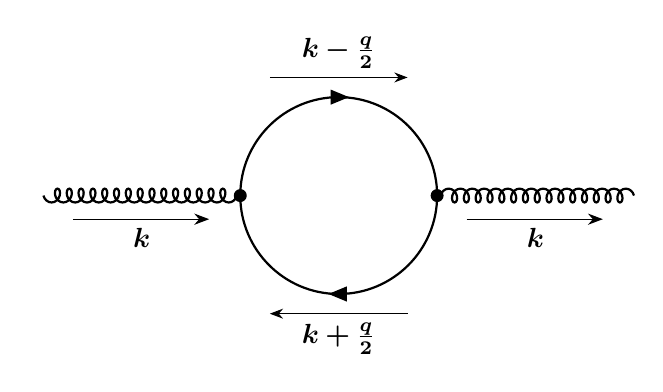
\begin{tikzpicture}
	
	\begin{feynman}
	
	% ------------------------------------------------
	% Ensure the dimensions of graphic are appropriate
	%\useasboundingbox (0, 0.7*\loopsh) rectangle (\loopsw, -0.7*\loopsh);
	
	% ------------------------------------------------
	% Relevant coordinates
	\coordinate (Beg) at (0.20cm,0);
	
	\path (Beg) +(2.50cm,0) coordinate (V1);
	\path (V1)  +(2.50cm,0) coordinate (V2);
	\path (V2)  +(2.50cm,0) coordinate (End);
	
	\path (V1)				+(0.00cm,1.20cm) coordinate (LabelStartUpper);
	\path (LabelStartUpper)	+(2.50cm,0.00cm) coordinate (LabelEndUpper);
	
	\path (V1)				+(0.00cm,-1.20cm) coordinate (LabelStartLower);
	\path (LabelStartLower)	+(2.50cm,0.00cm) coordinate (LabelEndLower);
	
	% ----------------
	% Dotted vertices
	\node[dot] (V1Dot) at (V1) +(0.00cm, 0.00cm);
	\node[dot] (V2Dot) at (V2) +(0.00cm, 0.00cm);
	
	%%%%%%%%%%%%%%%%%%%%%%%%%%%%%%%%%%%%%%%%%
	%Diagram
	\diagram*{
		
		(Beg)	-- [thick, gluon, momentum' = \(\boldsymbol{k}\)] (V1), 
		(End)	-- [thick, gluon, rmomentum = \(\boldsymbol{k}\)] (V2),
		
		(LabelStartUpper) -- [opacity=0, momentum = \(\boldsymbol{k-\frac{q}{2}}\)] (LabelEndUpper),
		
		(LabelStartLower) -- [opacity=0, rmomentum' = \(\boldsymbol{k+\frac{q}{2}}\)] (LabelEndLower),
		
	};
	
	\draw[thick, fermion] (V1) arc [start angle=180, end angle=0, radius=1.25cm];
	\draw[thick, fermion] (V2) arc [start angle=0, end angle=-180, radius=1.25cm];
	
		
	\end{feynman}
	
\end{tikzpicture}

% Set this figure's name when externalised 
\tikzsetnextfilename{qcdloops-ghostloop} 
%
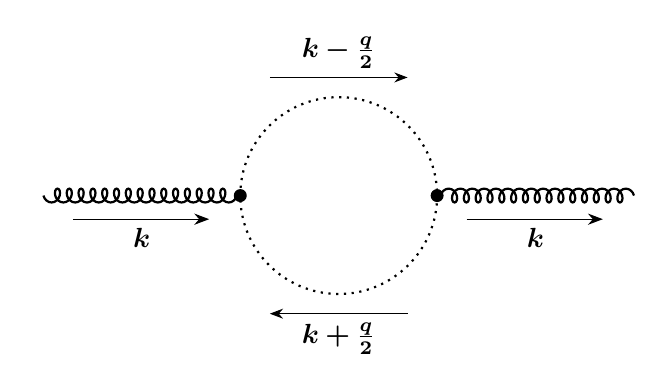
\begin{tikzpicture}
	
	\begin{feynman}
		
	% ------------------------------------------------
	% Ensure the dimensions of graphic are appropriate
	%\useasboundingbox (0, 0.7*\loopsh) rectangle (\loopsw, -0.7*\loopsh);
	
	% ------------------------------------------------
	% Relevant coordinates
	\coordinate (Beg) at (0.20cm,0);
	
	\path (Beg) +(2.50cm,0) coordinate (V1);
	\path (V1)  +(2.50cm,0) coordinate (V2);
	\path (V2)  +(2.50cm,0) coordinate (End);
	
	\path (V1)				+(0.00cm,1.20cm) coordinate (LabelStartUpper);
	\path (LabelStartUpper)	+(2.50cm,0.00cm) coordinate (LabelEndUpper);
	
	\path (V1)				+(0.00cm,-1.20cm) coordinate (LabelStartLower);
	\path (LabelStartLower)	+(2.50cm,0.00cm) coordinate (LabelEndLower);
	
	% ----------------
	% Dotted vertices
	\node[dot] (V1Dot) at (V1) +(0.00cm, 0.00cm);
	\node[dot] (V2Dot) at (V2) +(0.00cm, 0.00cm);
	
	%%%%%%%%%%%%%%%%%%%%%%%%%%%%%%%%%%%%%%%%%
	%Diagram
	\diagram*{
		
		(Beg)	-- [thick, gluon, momentum' = \(\boldsymbol{k}\)] (V1), 
		(End)	-- [thick, gluon, rmomentum = \(\boldsymbol{k}\)] (V2),
		
		(LabelStartUpper) -- [opacity=0, momentum = \(\boldsymbol{k-\frac{q}{2}}\)] (LabelEndUpper),
		
		(LabelStartLower) -- [opacity=0, rmomentum' = \(\boldsymbol{k+\frac{q}{2}}\)] (LabelEndLower),
		
	};
	
	\draw[very thick, ghost] (V1) arc [start angle=180, end angle=0, radius=1.25cm];
	\draw[very thick, ghost] (V2) arc [start angle=0, end angle=-180, radius=1.25cm];
	
		
	\end{feynman}
	
\end{tikzpicture}

% Set this figure's name when externalised 
\tikzsetnextfilename{qcdloops-gluontadpole} 
%
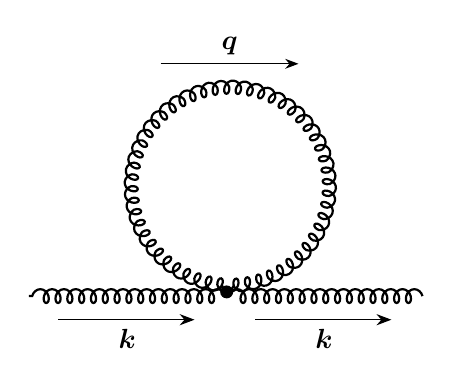
\begin{tikzpicture}
	
	\begin{feynman}
	
	% ------------------------------------------------
	% Ensure the dimensions of graphic are appropriate
	%\useasboundingbox (0, 0.7*\loopsh) rectangle (\loopsw, -0.7*\loopsh);
	
	% ------------------------------------------------
	% Relevant coordinates
	\coordinate (Beg) at (0.20cm,0);
	
	\path (Beg) +(2.50cm,0) coordinate (V1);
	\path (V1)  +(2.50cm,0) coordinate (End);
	
	% Loop should start slightly above line
	\path (V1)	+(-0.05cm,0.15cm) coordinate (V1LoopStart);
	
	% Loop Label
	\path (V1LoopStart)	+(-1.15cm,2.50cm) coordinate (LabelStart);
	\path (LabelStart)	+( 2.50cm,0.00cm) coordinate (LabelEnd);
		
	%%%%%%%%%%%%%%%%%%%%%%%%%%%%%%%%%%%%%%%%%		
	%Diagram
	\diagram*{
						
		(V1)	-- [thick, gluon, rmomentum = \(\boldsymbol{k}\)] (Beg),
		(End)	-- [thick, gluon, rmomentum = \(\boldsymbol{k}\)] (V1),
	
		(LabelStart) -- [opacity=0, momentum = \(\boldsymbol{q}\)] (LabelEnd),
	
	};
	
	% Draw the loop
	%\draw[<options>] (x,y) arc (start:stop:radius);
	\draw[thick, gluon] (V1LoopStart) arc (-95:272:1.25cm);
	
	% Draw the vertex dot
	\node[dot, above right = 0.00cm and -0.04cm of V1] (Dot);
		
	\end{feynman}
	
\end{tikzpicture}

% Set this figure's name when externalised 
\tikzsetnextfilename{qcdloops-vertexghostgluon-ghostexchange} 
%
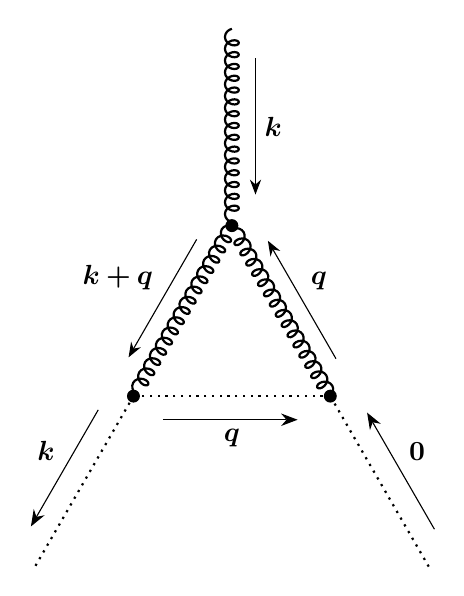
\begin{tikzpicture}
	
	\begin{feynman}
	
	% ------------------------------------------------
	% Ensure the dimensions of graphic are appropriate
	%\useasboundingbox (0, 0.7*\loopsh) rectangle (\loopsw, -0.7*\loopsh);
	
	% ------------------------------------------------
	% Relevant coordinates
	\coordinate (Beg) at (0,0);
	
	\path (Beg) +(0,-2.50cm) coordinate (VU);
	\path (VU)  +(300:2.50cm) coordinate (VR);
	\path (VU)  +(240:2.50cm) coordinate (VL);
		
	\path (VR)  +(300:2.50cm) coordinate (GhostR);
	\path (VL)  +(240:2.50cm) coordinate (GhostL);
		
	% ----------------
	% Dotted vertices
	\node[dot] (VUDot) at (VU) +(0.00cm, 0.00cm);
	\node[dot] (VLDot) at (VL) +(0.00cm, 0.00cm);
	\node[dot] (VRDot) at (VR) +(0.00cm, 0.00cm);
	
	%%%%%%%%%%%%%%%%%%%%%%%%%%%%%%%%%%%%%%%%%
	%Diagram
	\diagram*{
	
	(Beg) -- [thick, gluon, momentum = \(\boldsymbol{k}\)] (VU),
	
	(VU) --	[thick, gluon, momentum' = \(\boldsymbol{k+q}\)] (VL)
		 -- [very thick, ghost, momentum' = \(\boldsymbol{k}\)] (GhostL),		
		 
	(GhostR) -- [very thick, ghost, momentum' = \(\boldsymbol{0}\)] (VR)
			 -- [thick, gluon, momentum' = \(\boldsymbol{q}\)] (VU),
		 
	(VR) -- [very thick, ghost, rmomentum = \(\boldsymbol{q}\)] (VL),	 
		 
	};
	
	
	\end{feynman}
	
\end{tikzpicture}

% Set this figure's name when externalised 
\tikzsetnextfilename{qcdloops-vertexghostgluon-gluonexchange} 
%
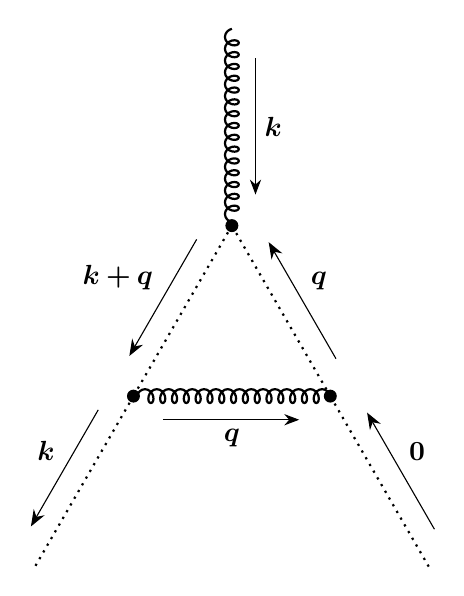
\begin{tikzpicture}
	
	\begin{feynman}
	
	% ------------------------------------------------
	% Ensure the dimensions of graphic are appropriate
	%\useasboundingbox (0, 0.7*\loopsh) rectangle (\loopsw, -0.7*\loopsh);
	
	% ------------------------------------------------
	% Relevant coordinates
	\coordinate (Beg) at (0,0);
	
	\path (Beg) +(0,-2.50cm) coordinate (VU);
	\path (VU)  +(300:2.50cm) coordinate (VR);
	\path (VU)  +(240:2.50cm) coordinate (VL);
	
	\path (VR)  +(300:2.50cm) coordinate (GhostR);
	\path (VL)  +(240:2.50cm) coordinate (GhostL);
	
	% ----------------
	% Dotted vertices
	\node[dot] (VUDot) at (VU) +(0.00cm, 0.00cm);
	\node[dot] (VLDot) at (VL) +(0.00cm, 0.00cm);
	\node[dot] (VRDot) at (VR) +(0.00cm, 0.00cm);
	
	%%%%%%%%%%%%%%%%%%%%%%%%%%%%%%%%%%%%%%%%%
	%Diagram
	\diagram*{
		
		(Beg) -- [thick, gluon, momentum = \(\boldsymbol{k}\)] (VU),
		
		(VU) --	[very thick, ghost, momentum' = \(\boldsymbol{k+q}\)] (VL)
			 -- [very thick, ghost, momentum' = \(\boldsymbol{k}\)] (GhostL),		
		
		(GhostR) -- [very thick, ghost, momentum' = \(\boldsymbol{0}\)] (VR)
				 -- [very thick, ghost, momentum' = \(\boldsymbol{q}\)] (VU),
		
		(VR) -- [thick, gluon, rmomentum = \(\boldsymbol{q}\)] (VL),	 
		
	};
	
		
	\end{feynman}
	
\end{tikzpicture}

\end{center}

\newpage


%%%%%%%%%%%%%%%%%%%%%%%%%%%%%%%%%%%%%%
% THE DOUBLE GLUON EMISSION DIAGRAMS
%%%%%%%%%%%%%%%%%%%%%%%%%%%%%%%%%%%%%%

\subsection{Double Gluon Emission Diagrams}

% NOTE: THESE ARE USED TO DETERMINE BOUNDING BOXES
% 		MUST BE DEFINED HERE

\begin{center}
	
\newlength{\imagew}\setlength{\imagew}{10.50cm}
\newlength{\imageh}\setlength{\imageh}{4.00cm}

% Set this figure's name when externalised 
\tikzsetnextfilename{thesis-doublesplitting-M1} 
%
\begin{tikzpicture}
    
    % ------------------------------------------------
    % Ensure the dimensions of graphic are appropriate
    \useasboundingbox (0, 0.5*\imageh) rectangle (\imagew, -0.5*\imageh);
    
    % NOTE: MUST *NOT* INCLUDE A {} LABEL FOR THIS ONE
    %		IF A LABEL IS PROVIDED, THERE WILL BE A WHITE CIRCLE OVER THE VERTEX 
    \coordinate (Blob) at (1.50cm, -0.75cm);

    \path (Blob) +(1.00cm, 0.00cm) coordinate (Mother);	        
    
    % Specify the quark endpoints
    \path (Mother) +(2.50cm,0.00cm) coordinate (Emission1);
    \path (Mother) +(5.00cm,0.00cm) coordinate (Emission2);
    \path (Mother) +(7.50cm,0.00cm) coordinate (Final);

	% Specify gluon endpoints
	% NOTE: Here, we use relative polar coordinates
	\path (Emission1) +(40:3.00cm) coordinate (Gluon1); % 30 degrees, 2.50 cm away from Emission1
	\path (Emission2) +(40:3.00cm) coordinate (Gluon2); 
    
    %%%%%%%%%%%%%%%%%%%%%%%%%%%%%%%%%%%%%%%%%%%%%%%
    \begin{feynman}

	% Diagram
	\diagram*{ %ALWAYS END LINES WITH A COMMA
	
	(Mother) 	-- [thick, fermion, momentum'=\( \boldsymbol{ p_{i}^{}} \)] (Emission1)
			 	-- [thick, fermion, momentum'=\( \boldsymbol{ q_{1}^{}} \)] (Emission2)
			 	-- [thick, fermion, momentum'=\( \boldsymbol{ p_{f}^{}} \)] (Final),
	
	(Gluon1) 	-- [thick, gluon, rmomentum' = \( \boldsymbol{k_{1}^{}} \)] (Emission1),

	(Gluon2) 	-- [thick, gluon, rmomentum' = \( \boldsymbol{k_{2}^{}} \)] (Emission2),
	
	};
	
    % The Blob
    % Called last so it overlaps with the fermion line
	\vertex[blob] (m) at (Blob) {\scalebox{2.0}{$\mathcal{M}^{ }_{\it h}$}}; 

    \end{feynman}    

\end{tikzpicture}

% Set this figure's name when externalised 
\tikzsetnextfilename{thesis-doublesplitting-M2} 
%
\begin{tikzpicture}

	% ------------------------------------------------
	% Ensure the dimensions of graphic are appropriate
	\useasboundingbox (0, 0.5*\imageh) rectangle (\imagew, -0.5*\imageh);
	
	% NOTE: MUST *NOT* INCLUDE A {} LABEL FOR THIS ONE
	%		IF A LABEL IS PROVIDED, THERE WILL BE A WHITE CIRCLE OVER THE VERTEX 
	\coordinate (Blob) at (1.50cm, -0.75cm);
	
	\path (Blob) +(1.00cm, 0.00cm) coordinate (Mother);	        
    
    % Specify the quark endpoints
    \path (Mother) +(2.50cm,0.00cm) coordinate (Emission1);
    \path (Mother) +(5.00cm,0.00cm) coordinate (Emission2);
    \path (Mother) +(7.50cm,0.00cm) coordinate (Final);

	% Specify gluon endpoints
	% NOTE: Here, we use relative polar coordinates

	% Gluon labeled k2
	\path (Emission1) +(10:5.00cm) coordinate (Gluon2); % 30 degrees, 2.50 cm away from (Emission1)

	% The arrow for momentum k2
	\path (Emission1) 	+(10:3.00cm) coordinate (ArrowStart2);
	\path (ArrowStart2) +(10:2.50cm) coordinate (ArrowEnd2);

	% Gluon labeled k1
	\path (Emission2) +(65:2.50cm) coordinate (Gluon1);

	% The arrow for momentum k1
	\path (Emission2) 	+(65:0.70cm) coordinate (ArrowStart1);
	\path (ArrowStart1) +(65:2.00cm) coordinate (ArrowEnd1);

    
    %%%%%%%%%%%%%%%%%%%%%%%%%%%%%%%%%%%%%%%%%%%%%%%
    \begin{feynman}
        		    	
	% Diagram
	\diagram*{ %ALWAYS END LINES WITH A COMMA
	
	(Mother) 	-- [thick, fermion, momentum'=\( \boldsymbol{ p_{i}^{}} \)] (Emission1)
			 	-- [thick, fermion, momentum'=\( \boldsymbol{ q_{2}^{}} \)] (Emission2)
			 	-- [thick, fermion, momentum'=\( \boldsymbol{ p_{f}^{}} \)] (Final),

	% This separation happens to avoid overlaps
	(ArrowStart2)	-- [white, momentum = \( \boldsymbol{k_{2}^{}} \)] (ArrowEnd2),
	(Gluon2)		-- [thick, gluon] (Emission1),


	(ArrowStart1)	-- [white, momentum = \( \boldsymbol{k_{1}^{}} \)] (ArrowEnd1),
	(Gluon1)		-- [thick, gluon] (Emission2),
	
	};

    % The Blob
	\vertex[blob] (m) at (Blob) {\scalebox{2.0}{$\mathcal{M}^{ }_{\it h}$}}; 
	
    \end{feynman}  
  
\end{tikzpicture}

% Set this figure's name when externalised 
\tikzsetnextfilename{thesis-doublesplitting-M3} 
%
\begin{tikzpicture}
	
	% ------------------------------------------------
	% Ensure the dimensions of graphic are appropriate
	\useasboundingbox (0, 0.5*\imageh) rectangle (\imagew, -0.5*\imageh);
	
	% NOTE: MUST *NOT* INCLUDE A {} LABEL FOR THIS ONE
	%		IF A LABEL IS PROVIDED, THERE WILL BE A WHITE CIRCLE OVER THE VERTEX 
	\coordinate (Blob) at (1.50cm, -0.75cm);
	
	\path (Blob) +(1.00cm, 0.00cm) coordinate (Mother);	        
	
	% Specify the quark endpoints
	\path (Mother)	  +(3.00cm,0.00cm)	coordinate (Emission1);
	\path (Emission1) +(25:2.50cm)		coordinate (Emission2);
	\path (Mother)    +(7.00cm,0.00cm)	coordinate (Final);
	
	% Specify gluon endpoints
	% NOTE: Here, we use relative polar coordinates
	\path (Emission2) +(30:2.50cm) coordinate (Gluon1); % 30 degrees, 2.50 cm away from Emission1
	\path (Emission2) +(00:2.50cm) coordinate (Gluon2); 
	
	%%%%%%%%%%%%%%%%%%%%%%%%%%%%%%%%%%%%%%%%%%%%%%%
	\begin{feynman}
		
		% Diagram
		\diagram*{ %ALWAYS END LINES WITH A COMMA
			
			(Mother) 	-- [thick, fermion, momentum'=\( \boldsymbol{ p_{i}^{}} \)] (Emission1)
						-- [thick, fermion, momentum'=\( \boldsymbol{ p_{f}^{}} \)] (Final),

			(Emission2) -- [thick, gluon, rmomentum' = \( \boldsymbol{q_{3}^{}} \)] (Emission1),

			(Gluon1) -- [thick, gluon, rmomentum' = \( \boldsymbol{k_{1}^{}} \)] (Emission2),
			(Gluon2) -- [thick, gluon, rmomentum = \( \boldsymbol{k_{2}^{}} \)] (Emission2),
						
		};
		
		% The Blob
		\vertex[blob] (m) at (Blob) {\scalebox{2.0}{$\mathcal{M}^{ }_{\it h}$}}; 
		
	\end{feynman}    
	
\end{tikzpicture}

% Set this figure's name when externalised 
\tikzsetnextfilename{thesis-doublesplitting-M4} 
%
\begin{tikzpicture}
		
	% ------------------------------------------------
	% Ensure the dimensions of graphic are appropriate
	\useasboundingbox (0, 0.5*\imageh) rectangle (\imagew, -0.5*\imageh);
	
	% NOTE: MUST *NOT* INCLUDE A {} LABEL FOR THIS ONE
	%		IF A LABEL IS PROVIDED, THERE WILL BE A WHITE CIRCLE OVER THE VERTEX 
	\coordinate (Blob) at (1.50cm, -0.75cm);
	
	\path (Blob) +(1.00cm, 0.00cm) coordinate (Mother);	        
	
	% Specify the quark endpoints
	\path (Mother)	  +(3.00cm,0.00cm)	coordinate (Emission1);
	\path (Emission1) +(25:2.50cm)		coordinate (Emission2);
	\path (Mother)    +(7.00cm,0.00cm)	coordinate (Final);
	
	% Specify gluon endpoints
	% NOTE: Here, we use relative polar coordinates
	\path (Emission2) +(30:2.50cm) coordinate (Ghost1); % 30 degrees, 2.50 cm away from Emission1
	\path (Emission2) +(00:2.50cm) coordinate (Ghost2); 
	
	%%%%%%%%%%%%%%%%%%%%%%%%%%%%%%%%%%%%%%%%%%%%%%%
	\begin{feynman}
		
		% Diagram
		\diagram*{ %ALWAYS END LINES WITH A COMMA
			
		(Mother) 	-- [thick, fermion, momentum'=\( \boldsymbol{ p_{i}^{}} \)] (Emission1)
						-- [thick, fermion, momentum'=\( \boldsymbol{ p_{f}^{}} \)] (Final),
			
		(Emission2) -- [thick, gluon, rmomentum' = \( \boldsymbol{q_{4}^{}} \)] (Emission1),
			
		(Emission2) -- [very thick, ghost, momentum = \( \boldsymbol{k_{1}^{}} \)] (Ghost1),
		(Ghost2) 	-- [very thick, ghost, rmomentum = \( \boldsymbol{k_{2}^{}} \)] (Emission2),
			
		};
		
		% The Blob
		\vertex[blob] (m) at (Blob) {\scalebox{2.0}{$\mathcal{M}^{ }_{\it h}$}}; 
		
	\end{feynman}    
		
\end{tikzpicture}

\end{center}



\newpage

%%%%%%%%%%%%%%%%%%%%%%%%%%%%%%%%%%%%%%
% PARTON SHOWER IN MEDIUM
%%%%%%%%%%%%%%%%%%%%%%%%%%%%%%%%%%%%%%

\subsection{Quark-Antiquark Antenna}

\begin{center}
	
% Set this figure's name when externalised 
\tikzsetnextfilename{qcd-antenna-lower} 
%
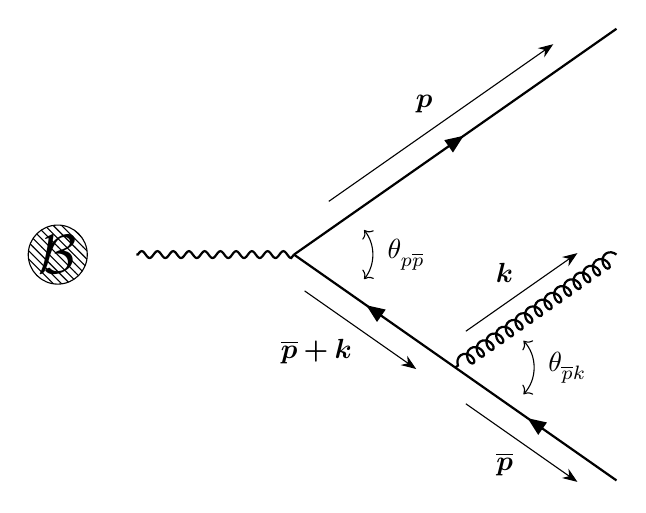
\begin{tikzpicture}
\begin{feynman}
		
	% ---------------------
	% Blob & Shower origin
	\coordinate (Blob) at (1.20cm,0.00cm);
	\path (Blob) +(1.00cm,0.00cm) coordinate (Origin);
	
	\path (Origin) +(2.00cm,0.00cm) coordinate (PairCreation);

	\path (PairCreation) +(+35:5.00cm) coordinate (Quark);	

	\path (PairCreation) +(-35:2.50cm) coordinate (Emission);
	\path (Emission) 	 +(-35:2.50cm) coordinate (AntiQuark);
	
	\path (Emission) +(+35:2.50cm) coordinate (Gluon);
	
	% ---------------------	
	\diagram*{
		
		(Origin) -- [thick, photon] (PairCreation),
		
		(AntiQuark) -- [thick, fermion, rmomentum = \(\boldsymbol{\overline{p}}\)] (Emission)
					-- [thick, fermion, rmomentum = \(\boldsymbol{\overline{p}+k}\)] (PairCreation)
					-- [thick, fermion, momentum  = \(\boldsymbol{p}\)] 			(Quark),
		
		(Gluon) -- [thick, gluon, rmomentum' = \(\boldsymbol{k}\)] (Emission),
		
	};
	
	% ------------------------------------------------
	% Blob Drawing
	\vertex[blob] (b) at (Blob) {\scalebox{2.00}{$\mathcal{B}$}}; 
	
	% ------------------------------------------------
	% Angles
	\path (PairCreation) +(0:0.50cm) coordinate (PairCreationAngle);
	\pic [draw, <->, "$\quad\theta\sub{p\overline{p}}$", angle eccentricity=1.5] {angle = AntiQuark--PairCreationAngle--Quark};    
	
	\path (Emission) +(0:0.50cm) coordinate (EmissionAngle);
	\pic [draw, <->, "$\quad\theta\sub{\overline{p}k}$", angle eccentricity=1.5] {angle = AntiQuark--EmissionAngle--Gluon};    
	
	
		
\end{feynman}
\end{tikzpicture}

% Set this figure's name when externalised 
\tikzsetnextfilename{qcd-antenna-upper} 
%
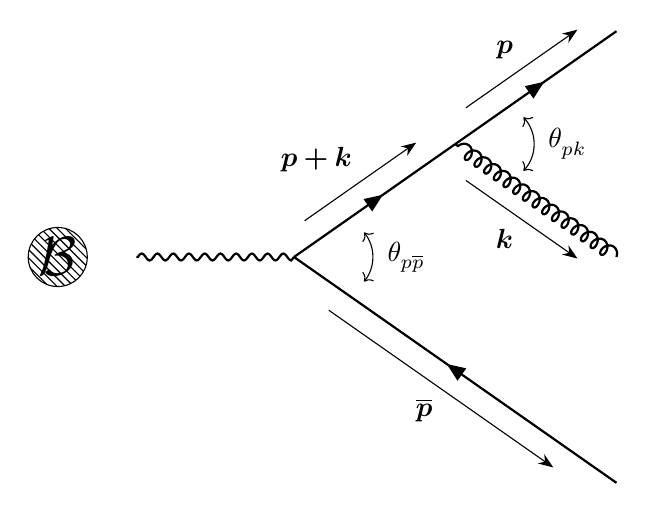
\begin{tikzpicture}
\begin{feynman}

	% ---------------------
	% Blob & Shower origin
	\coordinate (Blob) at (1.20cm,0.00cm);
	\path (Blob) +(1.00cm,0.00cm) coordinate (Origin);

	\path (Origin) +(2.00cm,0.00cm) coordinate (PairCreation);

	\path (PairCreation) +(+35:2.50cm) coordinate (Emission);
	\path (Emission) 	 +(+35:2.50cm) coordinate (Quark);
	
	\path (PairCreation) +(-35:5.00cm) coordinate (AntiQuark);
	
	\path (Emission) +(-35:2.50cm) coordinate (Gluon);



	% ---------------------	
	\diagram*{
	
	(Origin) -- [thick, photon] (PairCreation),
	
	(AntiQuark) -- [thick, fermion, rmomentum = \(\boldsymbol{\overline{p}}\)] (PairCreation)
				-- [thick, fermion, momentum  = \(\boldsymbol{p+k}\)] 			(Emission)
				-- [thick, fermion, momentum  = \(\boldsymbol{p}\)] 			(Quark),
				
	(Gluon) -- [thick, gluon, rmomentum = \(\boldsymbol{k}\)] (Emission),
	
	};

    % ------------------------------------------------
	% Blob Drawing
	\vertex[blob] (b) at (Blob) {\scalebox{2.00}{$\mathcal{B}$}}; 

	% ------------------------------------------------
	% Angles
	\path (PairCreation) +(0:0.50cm) coordinate (PairCreationAngle);
	\pic [draw, <->, "$\quad\theta\sub{p\overline{p}}$", angle eccentricity=1.5] {angle = AntiQuark--PairCreationAngle--Quark};    

	\path (Emission) +(0:0.50cm) coordinate (EmissionAngle);
	\pic [draw, <->, "$\quad\theta\sub{pk}$", angle eccentricity=1.5] {angle = Gluon--EmissionAngle--Quark};    
	

	
\end{feynman}\end{tikzpicture}

\end{center}


%%%%%%%%%%%%%%%%%%%%%%%%%%%%%%%%%%%%%%
% PARTON SPLITTINGS
%%%%%%%%%%%%%%%%%%%%%%%%%%%%%%%%%%%%%%

\subsection{Factorisation of Parton Splittings}

\begin{center}

% Set this figure's name when externalised 
\tikzsetnextfilename{factorisation-in} 
%
\begin{tikzpicture}
    \begin{feynman}
    
    %Vertices
    \vertex (Mother) {\( x\sub{\rm in} \) } ;
    
    \vertex [above right = +0.00 cm and +3.00 cm of Mother] (Vertex);
    
    \vertex [above right = +1.50 cm and +3.00 cm of Vertex] (Daughter1);
    \vertex [above right = -1.50 cm and +3.00 cm of Vertex] (Daughter2);

    %FOR THE DASHES
    \vertex [above right = +2.00 cm and +1.20 cm of Mother] (LeftUpp) {\(\mu\upp{2} + \delta\mu\upp{2}\)};
    \vertex [above right = -2.00 cm and +1.20 cm of Mother] (LeftLow);
    \vertex [above right = +0.00 cm and +4.20 cm of LeftUpp] (RightUpp) {\(\mu\upp{2}\)};
    \vertex [above right = +0.00 cm and +4.20 cm of LeftLow] (RightLow);


    %Diagram
    \diagram*{ %ALWAYS END LINES WITH A COMMA
    %(E,\boldsymbol{p_{ }^{}})
    (Mother) -- [thick, edge label = { \( i \) } ] (Vertex), 
                
    (Vertex) -- [thick, edge label = { \( a \) } ] (Daughter1), 

    (Vertex) -- [thick, edge label' = { \( j \) }] (Daughter2), 

    (LeftUpp) -- [thick, dashed] (LeftLow),
    (RightUpp) -- [thick, dashed] (RightLow),

    };
    
    \end{feynman}
    
    %-------------------------------------------
    %Labels
    
    \node[above right = -0.25 cm and 0.10 cm of Daughter1] (Daughter1Label) {\( x=z\,x\sub{\rm in} \)};

    \node[above right = -0.35 cm and 0.10 cm of Daughter2] (Daughter2Label) {\( (1-z)\,x\sub{\rm in} \)};

\end{tikzpicture}

% Set this figure's name when externalised 
\tikzsetnextfilename{factorisation-out} 
%
\begin{tikzpicture}
    \begin{feynman}
    
    %Vertices
    \vertex (Mother) {\( x \) } ;
    
    \vertex [above right = +0.00 cm and +3.00 cm of Mother] (Vertex);
    
    \vertex [above right = +1.50 cm and +3.00 cm of Vertex] (Daughter1);
    \vertex [above right = -1.50 cm and +3.00 cm of Vertex] (Daughter2);

    %FOR THE DASHES
    \vertex [above right = +2.00 cm and +1.20 cm of Mother] (LeftUpp) {\(\mu\upp{2} + \delta\mu\upp{2}\)};
    \vertex [above right = -2.00 cm and +1.20 cm of Mother] (LeftLow);
    \vertex [above right = +0.00 cm and +4.20 cm of LeftUpp] (RightUpp) {\(\mu\upp{2}\)};
    \vertex [above right = +0.00 cm and +4.20 cm of LeftLow] (RightLow);


    %Diagram
    \diagram*{ %ALWAYS END LINES WITH A COMMA
    %(E,\boldsymbol{p_{ }^{}})
    (Mother) -- [thick, edge label = { \( a \) } ] (Vertex), 
                
    (Vertex) -- [thick, edge label = { \( j \) } ] (Daughter1), 

    (Vertex) -- [thick, edge label' = { \( k \) }] (Daughter2), 

    (LeftUpp) -- [thick, dashed] (LeftLow),
    (RightUpp) -- [thick, dashed] (RightLow),

    };
    
    \end{feynman}
    
    %-------------------------------------------
    %Labels
    
    \node[above right = -0.25 cm and 0.10 cm of Daughter1] (Daughter1Label) {\( x\sub{\rm out} = z\,x \)};

    \node[above right = -0.35 cm and 0.10 cm of Daughter2] (Daughter2Label) {\( (1-z)\,x \)};

\end{tikzpicture}
	
\end{center}

\newpage

%%%%%%%%%%%%%%%%%%%%%%%%%%%%%%%%%%%%%%
% PARTON SHOWER IN MEDIUM
%%%%%%%%%%%%%%%%%%%%%%%%%%%%%%%%%%%%%%

\subsection{Medium Parton Shower}

\begin{center}
	
% Set this figure's name when externalised 
%\tikzsetnextfilename{partonshowermedium-steps} 
\tikzsetnextfilename{partonshowermedium-full-highlight} 

%
\newlength{\QGPlength}\setlength{\QGPlength}{12.00cm}
\newlength{\QGPheight}\setlength{\QGPheight}{9.00cm}
%
% %%%%%%%%%%%%%%%%%%%%%%%%%%%%%%%%%%%%%%%%%%%%%%%%%%%%%%%%%%
% NOTE TO SELF:
% 	IN TEXSTUDIO, COMMENT MULTIPLE LINES AT ONCE WITH CTRL+T
% %%%%%%%%%%%%%%%%%%%%%%%%%%%%%%%%%%%%%%%%%%%%%%%%%%%%%%%%%%
%
\begin{tikzpicture}
\begin{feynman}
		
% Proper size --- Bounding box
\useasboundingbox (0, 0.5*\QGPheight) rectangle (\QGPlength, -0.5*\QGPheight);

% ------------------------------------------------
% COMMENT THESE LINES TO SEE THE INDIVIDUAL STEPS
% ------------------------------------------------	

% QGP Effect
\path[left color=orange!70,right color=white, overlay] (0, 0.5*\QGPheight) rectangle (\QGPlength, -0.5*\QGPheight);

% Vacuum emissions
% ---------------------
% Blob & Shower origin
\coordinate (Blob) at (1.20cm,0.00cm);
\path (Blob) +(1.00cm,0.00cm) coordinate (Origin);

% ------------------------------------------------
% Blob Drawing
\vertex[blob] (b) at (Blob) {}; 

% ------------------------------------------------
% Coordinates: Vacuum Shower 

\path (Origin) +(2.00cm,0.00cm) coordinate (PairCreation);

% Main Branches	
\path (PairCreation) +(+30:7.00cm) coordinate (EndUpperBranch);
\path (PairCreation) +(-30:7.00cm) coordinate (EndLowerBranch);

\path (EndUpperBranch) +(+20:1.50cm) coordinate (UpperGluon);
\path (EndUpperBranch) +(-40:1.50cm) coordinate (UpperFermion);

\path (EndLowerBranch) +(-35:1.50cm) coordinate (LowerGluon);
\path (EndLowerBranch) +(+20:1.50cm) coordinate (LowerFermion);

% 'First Emission' branch
\path (PairCreation) +(+30:0.75cm) coordinate (Emission1);
%
\path (Emission1) +(+00:2.50cm) coordinate (Gluon1);
%
\path (Gluon1) +(+15:2.00cm) coordinate (Gluon1a);
\path (Gluon1a) +(+10:2.50cm) coordinate (Fermion1a);
\path (Gluon1a) +(-10:2.50cm) coordinate (Fermion1b);
%
\path (Gluon1) +(-20:3.00cm) coordinate (Gluon1b);
\path (Gluon1b) +(+15:1.75cm) coordinate (Gluon1c);			
\path (Gluon1b) +(-15:1.75cm) coordinate (Gluon1d);			

% 'Second Emission' branch
\path (PairCreation) +(-30:5.25cm) coordinate (Emission2);
%
\path (Emission2) +(+20:2.00cm) coordinate (Gluon2);
%
\path (Gluon2) +(+15:1.00cm) coordinate (Fermion2a);	
\path (Gluon2) +(-10:1.00cm) coordinate (Fermion2b);	

% ------------------------------------------------
% Diagram: Vacuum Shower
\diagram*{
	
	% Main branches and pair creation 	
	(Origin) -- [photon] (PairCreation),
	
	(LowerFermion)	-- [fermion] (EndLowerBranch)
	-- [fermion] (PairCreation) 
	-- [fermion] (EndUpperBranch) 
	-- [fermion] (UpperFermion),
	
	(UpperGluon) -- [gluon] (EndUpperBranch),
	(LowerGluon) -- [gluon] (EndLowerBranch),
	
	% 'First Emission' branch
	(Emission1) -- [gluon] (Gluon1) 
	-- [gluon] {(Gluon1a), (Gluon1b)},
	
	(Fermion1b) -- [fermion] (Gluon1a)
	-- [fermion] (Fermion1a),
	
	{(Gluon1c), (Gluon1d)} -- [gluon] (Gluon1b),
	
	% 'Second Emission' branch
	
	(Emission2) -- [gluon] (Gluon2),
	
	(Fermion2a) -- [fermion] (Gluon2) 
	-- [fermion] (Fermion2b),
	
};

	
% Medium induced emissions
% ------------------------------------------------
% Coordinates: Medium-induced emissions

% Induced upper branch	
\path (PairCreation) +(+30:4.50cm) coordinate (InducedEmission1);
%
\path (InducedEmission1) +(-10:2.50cm) coordinate (InducedGluon1);
%
\path (InducedGluon1) +(+15:1.00cm) coordinate (InducedFermion1a);	
\path (InducedGluon1) +(-10:1.00cm) coordinate (InducedFermion1b);	

% Induced lower branch	
\path (PairCreation) +(-30:2.00cm) coordinate (InducedEmission2);
%
\path (InducedEmission2) +(-65:3.50cm) coordinate (InducedGluon2);


% ------------------------------------------------
% Diagram: Medium-induced emissions
\diagram*{
			
	% Induced upper branch	
	(InducedEmission1) -- [gluon] (InducedGluon1),
	
	(InducedFermion1a)	-- [fermion] (InducedGluon1) 
	-- [fermion] (InducedFermion1b),
	
	% Induced lower branch	
	(InducedGluon2) -- [gluon] (InducedEmission2),	

};

% Medium collisions
% ------------------------------------------------
% Coordinates: Medium collisions

% Upper branch collision
\path (PairCreation) +(+30:2.50cm) coordinate (CollEnd1);
%
\path (CollEnd1) +(90:0.90cm) coordinate (CollInit1);
%
\path (CollInit1) +(160:0.75cm) coordinate (CollIncoming1);	
\path (CollInit1) +(030:0.75cm) coordinate (CollOutgoing1);	

% Middle branch collision
\path (Gluon1) +(-20:1.50cm) coordinate (CollEnd2Aux);
\path (CollEnd2Aux) +(0cm,-0.08cm) coordinate (CollEnd2); % Because gluons curl
%
\path (CollEnd2) +(-90:0.90cm) coordinate (CollInit2);
%
\path (CollInit2) +(200:0.75cm) coordinate (CollIncoming2);	
\path (CollInit2) +(-30:0.75cm) coordinate (CollOutgoing2);		

% Lower branch collision
\path (PairCreation) +(-30:0.70cm) coordinate (CollEnd3);
%
\path (CollEnd3) +(-90:0.90cm) coordinate (CollInit3);
%
\path (CollInit3) +(200:0.75cm) coordinate (CollIncoming3);	
\path (CollInit3) +(-30:0.75cm) coordinate (CollOutgoing3);		

% ------------------------------------------------
% Diagram: Medium collisions

\diagram*{
	
	% Upper branch collision
	(CollEnd1) -- [gluon] (CollInit1),
	
	(CollIncoming1)	-- [fermion] (CollInit1) 
					-- [fermion] (CollOutgoing1),
	
	% Middle branch collision
	(CollEnd2) -- [gluon] (CollInit2),
	
	(CollIncoming2)	-- [fermion] (CollInit2) 
					-- [fermion] (CollOutgoing2),
	
	
	% Lower branch collision
	(CollEnd3) -- [gluon] (CollInit3),
	
	(CollIncoming3)	-- [fermion] (CollInit3) 
					-- [fermion] (CollOutgoing3),

};

% Medium Recoils
% ------------------------------------------------
% Coordinates: Medium recoil

\path (CollOutgoing1) +(120:0.70cm) coordinate (RecoilIncoming1);
\path (CollOutgoing1) +(005:1.30cm) coordinate (RecoilOutgoing1);

\path (CollOutgoing2) +(220:0.70cm) coordinate (RecoilIncoming2);
\path (CollOutgoing2) +(005:1.30cm) coordinate (RecoilOutgoing2);



% ------------------------------------------------
% Diagram: Medium recoil

\diagram*{

(RecoilIncoming1)	-- [gluon] (CollOutgoing1)
					-- [fermion] (RecoilOutgoing1),

(RecoilIncoming2)	-- [gluon] (CollOutgoing2)
					-- [fermion] (RecoilOutgoing2),


};

% ------------------------------------------------
% Medium recoils dot
\node[red,dot] (RD1) at (CollOutgoing1);
\node[red,dot] (RD2) at (CollOutgoing2);
	
			
\end{feynman}
\end{tikzpicture}

\end{center}


%%%%%%%%%%%%%%%%%%%%%%%%%%%%%%%%%%%%%%
% MEDIUM MODIFIED SPLITTING
%%%%%%%%%%%%%%%%%%%%%%%%%%%%%%%%%%%%%%

\subsection{Medium Modified Splitting}

\begin{center}
	
% Set this figure's name when externalised 
\tikzsetnextfilename{medium-modified-splitting} 
%
\newlength{\length}\setlength{\length}{12.50cm}
\newlength{\height}\setlength{\height}{14.00cm}

\begin{tikzpicture}
	\begin{feynman}
		
	% ---------------------
	% Proper size --- Bounding box
	\useasboundingbox (0, 0.5*\height) rectangle (\length, -0.5*\height);	

	% ----------------
	% M and MDagger
		
	% ---------------------
% Blob & Shower origin
\coordinate (Blob) at (2.50cm,3.00cm);
\path (Blob) +(1.00cm,0.00cm) coordinate (Origin); % Just outside the blob

% ------------------------------------------------
% Blob Drawing
\vertex[blob, thick] (b) at (Blob) {}; 

% ------------------------------------------------
% Splitting
\path (Origin)		+(+00:2.00cm) coordinate (Emission);
\path (Emission)	+(+25:6.50cm) coordinate (GluonEnd);
\path (Emission)	+(-10:6.50cm) coordinate (QuarkEnd);

\node[black,dot] (v) at (Emission);

% ------------------------------------------------
% ------------------------------------------------
% ------------------------------------------------
% Medium modifications


% ----------------------------
% A loop for pre-emission interactions

\path (Origin) +(0.40cm,-0.85cm) coordinate (A1);
\vertex[crossed dot, thick] (a1) at (A1) {};

\path (A1) +(0.00cm,+0.15cm) coordinate (As1);
\path (A1) +(0.00cm,+0.85cm) coordinate (Ae1);

\foreach \i in {2}
{
	
	\pgfmathtruncatemacro{\prev}{\i - 1}; % Compute previous index #RealProgrammingLanguage
	
	\path (A\prev) +(+00:1.20cm) coordinate (A\i); % Next scattering centre
	
	\vertex[crossed dot, thick] (a) at (A\i) {}; % Draw crossed dot
	
	\path (A\i) +(0.00cm,+0.15cm) coordinate (As\i); % Start of exchanged gluons
	\path (A\i) +(0.00cm,+0.85cm) coordinate (Ae\i); % End of exchanged gluons
	
}

% ----------------------------
% A loop for post-emission interactions

% The first quark-medium scattering
\path (Emission) +(0.70cm,-1.00cm) coordinate (Q1);
\vertex[crossed dot, thick] (q) at (Q1) {};

\path (Q1) +(0.00cm,+0.15cm) coordinate (Qs1); % Start of exchanged gluon
\path (Q1) +(0.00cm,+0.87cm) coordinate (Qe1); % End of exchanged gluon

% The first gluon-medium scattering
\path (Emission) +(0.70cm,+1.50cm) coordinate (G1);
\vertex[crossed dot, thick] (g) at (G1) {};

\path (G1) +(0.00cm,-0.15cm) coordinate (Gs1); % Start of exchanged gluon
\path (G1) +(0.00cm,-1.07cm) coordinate (Ge1); % End of exchanged gluon

% ----------
% A LOOP !!!
\foreach \i in {2,...,5}
{

\pgfmathtruncatemacro{\prev}{\i - 1}; % Compute previous index #RealProgrammingLanguage

% -----------
% QUARK

\path (Q\prev) +(-10:1.20cm) coordinate (Q\i); % Next scattering centre

\vertex[crossed dot, thick] (q) at (Q\i) {}; % Draw crossed dot

\path (Q\i) +(0.00cm,+0.15cm) coordinate (Qs\i); % Start of exchanged gluons
\path (Q\i) +(0.00cm,+0.87cm) coordinate (Qe\i); % End of exchanged gluons

% -----------
% GLUON

\path (G\prev) +(+25:1.20cm) coordinate (G\i); % Next scattering centre

\vertex[crossed dot, thick] (g) at (G\i) {}; % Draw crossed dot

\path (G\i) +(0.00cm,-0.15cm) coordinate (Gs\i); % Start of exchanged gluons
\path (G\i) +(0.00cm,-1.07cm) coordinate (Ge\i); % End of exchanged gluons

}



% ------------------------------------------------
% Diagram:
\diagram*{
	
	% --------
	% Emission	
	(Origin) -- [fermion, thick] (Emission) -- [fermion, thick] (QuarkEnd),
	(GluonEnd) -- [gluon, thick] (Emission),

	% --------
	% Scatterings	
	(As1) -- [gluon, thick] (Ae1),
	(As2) -- [gluon, thick] (Ae2),

	\foreach \i in {1,...,5}
	{ 
	(Qs\i) -- [gluon, thick] (Qe\i),	
	(Gs\i) -- [gluon, thick] (Ge\i),
	}	

};
	

	% ---------------------
% Blob & Shower origin
\coordinate (BlobDagger) at (2.50cm,-3.00cm);
\path (BlobDagger) +(1.00cm,0.00cm) coordinate (Origin); % Just outside the blob

% ------------------------------------------------
% Blob Drawing
\vertex[blob, thick] (b) at (BlobDagger) {}; 

% ------------------------------------------------
% Splitting
\path (Origin)		+(+00:4.50cm) coordinate (EmissionDagger);
\path (EmissionDagger)	+(+25:4.00cm) coordinate (GluonEnd);
\path (EmissionDagger)	+(-10:4.00cm) coordinate (QuarkEnd);

\node[black,dot] (v) at (EmissionDagger);

% ------------------------------------------------
% ------------------------------------------------
% ------------------------------------------------
% Medium modifications


% ----------------------------
% A loop for pre-emission interactions

\path (Origin) +(0.40cm,-0.85cm) coordinate (A1);
\vertex[crossed dot, thick] (a1) at (A1) {};

\path (A1) +(0.00cm,+0.15cm) coordinate (As1);
\path (A1) +(0.00cm,+0.85cm) coordinate (Ae1);

\foreach \i in {2,...,4}
{
	
	\pgfmathtruncatemacro{\prev}{\i - 1}; % Compute previous index #RealProgrammingLanguage
	
	\path (A\prev) +(+00:1.20cm) coordinate (A\i); % Next scattering centre
	
	\vertex[crossed dot, thick] (a) at (A\i) {}; % Draw crossed dot
	
	\path (A\i) +(0.00cm,+0.15cm) coordinate (As\i); % Start of exchanged gluons
	\path (A\i) +(0.00cm,+0.85cm) coordinate (Ae\i); % End of exchanged gluons
	
}

% ----------------------------
% A loop for post-emission interactions

% The first quark-medium scattering
\path (EmissionDagger) +(0.70cm,-1.00cm) coordinate (Q1);
\vertex[crossed dot, thick] (q) at (Q1) {};

\path (Q1) +(0.00cm,+0.15cm) coordinate (Qs1); % Start of exchanged gluon
\path (Q1) +(0.00cm,+0.87cm) coordinate (Qe1); % End of exchanged gluon

% The first gluon-medium scattering
\path (EmissionDagger) +(0.70cm,+1.50cm) coordinate (G1);
\vertex[crossed dot, thick] (g) at (G1) {};

\path (G1) +(0.00cm,-0.15cm) coordinate (Gs1); % Start of exchanged gluon
\path (G1) +(0.00cm,-1.10cm) coordinate (Ge1); % End of exchanged gluon

% ----------
% A LOOP !!!
\foreach \i in {2,...,3}
{
	
	\pgfmathtruncatemacro{\prev}{\i - 1}; % Compute previous index #RealProgrammingLanguage
	
	% -----------
	% QUARK
	
	\path (Q\prev) +(-10:1.20cm) coordinate (Q\i); % Next scattering centre
	
	\vertex[crossed dot, thick] (q) at (Q\i) {}; % Draw crossed dot
	
	\path (Q\i) +(0.00cm,+0.15cm) coordinate (Qs\i); % Start of exchanged gluons
	\path (Q\i) +(0.00cm,+0.87cm) coordinate (Qe\i); % End of exchanged gluons
	
	% -----------
	% GLUON
	
	\path (G\prev) +(+25:1.20cm) coordinate (G\i); % Next scattering centre
	
	\vertex[crossed dot, thick] (g) at (G\i) {}; % Draw crossed dot
	
	\path (G\i) +(0.00cm,-0.15cm) coordinate (Gs\i); % Start of exchanged gluons
	\path (G\i) +(0.00cm,-1.10cm) coordinate (Ge\i); % End of exchanged gluons
	
}



% ------------------------------------------------
% Diagram:
\diagram*{
	
	% --------
	% Emission	
	(Origin) -- [fermion, thick] (EmissionDagger) -- [fermion, thick] (QuarkEnd),
	(GluonEnd) -- [gluon, thick] (EmissionDagger),
	
	% --------
	% Scatterings	
	
	(As1) -- [gluon, thick] (Ae1),
	(As2) -- [gluon, thick] (Ae2),
	(As3) -- [gluon, thick] (Ae3),
	(As4) -- [gluon, thick] (Ae4),
	
	\foreach \i in {1,...,3}
	{ 
		(Qs\i) -- [gluon, thick] (Qe\i),	
		(Gs\i) -- [gluon, thick] (Ge\i),
	}	
	
};


	% ----------------
	% LABELS M
	\path (Blob)	+(-2.25cm,+0.00cm) coordinate (LabelM);
	\vertex at (LabelM) {\qquad \scalebox{1.5}{$\mathcal{M}\hphantom{\upp{\dagger}}:$}};

	\path (BlobDagger)	+(-2.25cm,+0.00cm) coordinate (LabelMDagger);
	\vertex at (LabelMDagger) {\qquad \scalebox{1.5}{$\mathcal{M}\upp{\dagger}:$}};

	
	% ----------------
	% LINES
	\path (Emission)		+(0.00cm,+3.00cm) coordinate (StartLineUp);
	\path (Emission)		+(0.00cm,-9.00cm) coordinate (StartLineDown);

	\path (EmissionDagger)	+(0.00cm,+9.00cm) coordinate (EndLineUp);
	\path (EmissionDagger)	+(0.00cm,-3.00cm) coordinate (EndLineDown);
		
	\draw[dashed, thick] (StartLineDown) -- (StartLineUp);
	\draw[dashed, thick] (EndLineDown) -- (EndLineUp);

	% ----------------
	% LABELS
	
	\path (StartLineUp)	+(-0.35cm,+0.30cm) coordinate (LabelT);
	\path (EndLineUp) 	+(-0.35cm,+0.30cm) coordinate (LabelTDagger);
	
	\vertex at (LabelT) {\qquad \scalebox{1.5}{$t$}};
	\vertex at (LabelTDagger) {\qquad \scalebox{1.5}{$t'$}};
		
	\end{feynman}
\end{tikzpicture}
	
\end{center}




%%%%%%%%%%%%%%%%%%%%%%%%%%%%%%%%%%%%%%
% A CONTOUR INTEGRAL --- FOR FUN!
%%%%%%%%%%%%%%%%%%%%%%%%%%%%%%%%%%%%%%

\subsection{Contour Integral}

\begin{center}

% Set this figure's name when externalised 
\tikzsetnextfilename{contour-integral} 
%
%%%%%%%%%%%%%%%%%%%%%%%
%%%% BLACK MAGIC  %%%%%
%%%% DO NOT TOUCH %%%%%
%%%%%%%%%%%%%%%%%%%%%%%
\usetikzlibrary{decorations.pathreplacing,decorations.markings}
%
\tikzset{
  % style to apply some styles to each segment of a path
  on each segment/.style={
    decorate,
    decoration={
      show path construction,
      moveto code={},
      lineto code={
        \path [#1]
        (\tikzinputsegmentfirst) -- (\tikzinputsegmentlast);
      },
      curveto code={
        \path [#1] (\tikzinputsegmentfirst)
        .. controls
        (\tikzinputsegmentsupporta) and (\tikzinputsegmentsupportb)
        ..
        (\tikzinputsegmentlast);
      },
      closepath code={
        \path [#1]
        (\tikzinputsegmentfirst) -- (\tikzinputsegmentlast);
      },
    },
  },
  % style to add an arrow in the middle of a path
  mid arrow/.style={postaction={decorate,decoration={
        markings,
        mark=at position .5 with {\arrow[#1]{stealth}}
      }}},
}
%%%%%%%%%%%%%%%%%%%%%%%
%%%%%%%%%%%%%%%%%%%%%%%
%%%%%%%%%%%%%%%%%%%%%%%
%%%%%%%%%%%%%%%%%%%%%%%

\begin{tikzpicture}[thick]
    % axes and points
    \draw
      (-3.5,0) edge[-latex] node[at end,right]{${\rm Re}\,k$} (4,0) %Horizontal axis
      (0,-3.5) edge[-latex] node[at end,right]{${\rm Im}\,k$} (0,4) %Vertical axis
      
      %Ensure symmetric borders
      (-4,+0) node(phantomx) {\phantom{${\rm Re} k$}}
      (+0,-4) node(phantomy) {\phantom{${\rm Im} k$}}
      
      (0,-1) node[scale=3](-i){.} node[left]{$-{\rm i}\,\varepsilon$} %Pole

      % For the circles
      (3,0)  coordinate(R) node[below]{}
      (-3,0) coordinate(-R) node[below]{}

    % For the shifted straight lines
      (+3,+0.0175)  coordinate(UpperR) node[below]{}
      (+0,-0.0175)  coordinate(UpperZero) node[below]{}
      (-3,+0.0175) coordinate(-UpperR) node[below]{}
      (+3,-0.0175)  coordinate(LowerR) node[below]{}
      (+0,-0.0175)  coordinate(LowerZero) node[below]{}
      (-3,-0.0175) coordinate(-LowerR) node[below]{}

    %% For labels
      (3.25,0.5) node[below]{$R$}
      (-3.35,0.5) node[below]{$-R$}

      (+2.0,+0.5) node[above]{\textcolor{Bittersweet}{$x<0$}}
      (+2.0,-0.5) node[below]{\textcolor{OliveGreen}{$x>0$}}
    ;
    % the path
    
    % Upper arc
    \draw[Bittersweet, very thick]
    (-R) arc(+180:+0:3cm)
    (-UpperR) -- (UpperR)
    ;
    
    %lower arc
    \draw[OliveGreen, very thick]
    (-R) arc(-180:+0:3cm)
    (-LowerR) -- (LowerR)
    ;

    %Upper Contour Arrows
    \path [Bittersweet, very thick,postaction={on each segment={mid arrow=Bittersweet}}]
    (R) arc(+0:+180:3cm)
    (-UpperR) -- (UpperZero)
    ;

    %Lower Contour Arrows
    \path [OliveGreen, very thick,postaction={on each segment={mid arrow=OliveGreen}}]
    (R) arc(+0:-180:3cm)
    (LowerZero) -- (LowerR) 
    ;

\end{tikzpicture}


\end{center}


\end{document}

